\documentclass{article}
\usepackage[utf8]{inputenc}
\usepackage{pgfplots}
\usepackage{pythontex}
\usepackage{subfigure}
\pgfplotsset{compat=1.5}
\date{May 2019}
\begin{document}
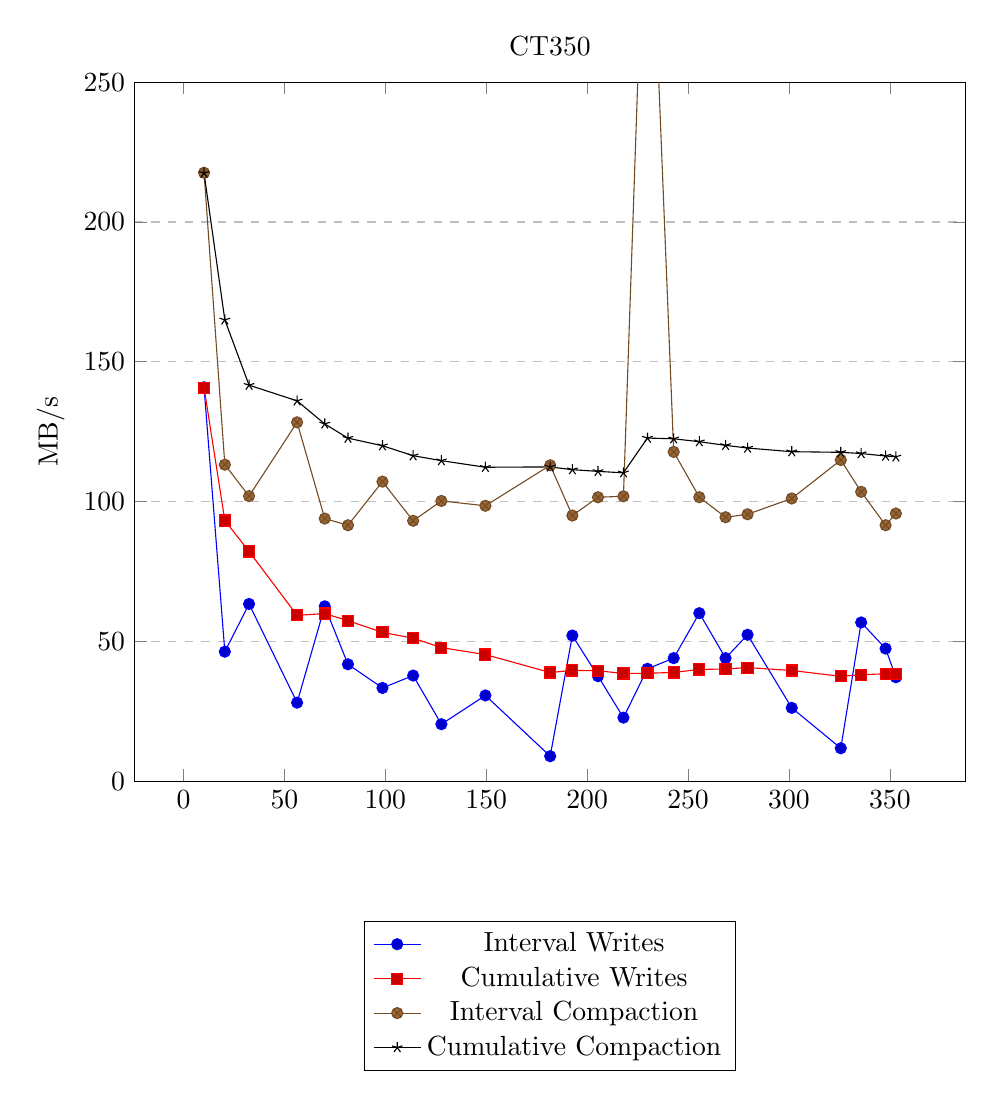
\begin{tikzpicture}
\begin{axis}[
title=CT350,
xlabel={},
ylabel={MB/s},
ymin=0,
ymax=250,
ytick={0,50,...,300},
width=\textwidth,
legend style={
    at={(0.5,-0.2)},
    anchor=north,legend columns=1
},
ymajorgrids=true,
grid style=dashed,
]
\addplot
	coordinates { (10.2,140.85)(20.5,46.30)(32.5,63.37)(56.3,28.07)(70.0,62.52)(81.5,41.79)(98.6,33.33)(113.8,37.77)(127.8,20.36)(149.6,30.65)(181.7,8.92)(192.7,52.08)(205.4,37.55)(218.0,22.71)(229.9,40.18)(242.9,43.99)(255.6,60.08)(268.6,44.00)(279.5,52.34)(301.4,26.21)(325.7,11.76)(335.8,56.76)(347.9,47.41)(353.0,37.16) };
\addplot
	coordinates { (10.2,140.76)(20.5,93.21)(32.5,82.16)(56.3,59.30)(70.0,59.93)(81.5,57.39)(98.6,53.20)(113.8,51.14)(127.8,47.76)(149.6,45.27)(181.7,38.85)(192.7,39.60)(205.4,39.48)(218.0,38.51)(229.9,38.59)(242.9,38.88)(255.6,39.94)(268.6,40.13)(279.5,40.61)(301.4,39.57)(325.7,37.49)(335.8,38.07)(347.9,38.39)(353.0,38.37) };
\addplot
	coordinates { (10.2,217.60)(20.5,113.19)(32.5,101.95)(56.3,128.34)(70.0,93.91)(81.5,91.52)(98.6,107.13)(113.8,93.12)(127.8,100.22)(149.6,98.49)(181.7,112.98)(192.7,95.00)(205.4,101.53)(218.0,101.89)(229.9,351.10)(242.9,117.77)(255.6,101.55)(268.6,94.39)(279.5,95.45)(301.4,101.10)(325.7,114.85)(335.8,103.48)(347.9,91.54)(353.0,95.72) };
\addplot
	coordinates { (10.2,217.46)(20.5,164.97)(32.5,141.63)(56.3,136.02)(70.0,127.76)(81.5,122.68)(98.6,119.97)(113.8,116.40)(127.8,114.62)(149.6,112.27)(181.7,112.39)(192.7,111.40)(205.4,110.79)(218.0,110.28)(229.9,122.71)(242.9,122.45)(255.6,121.41)(268.6,120.10)(279.5,119.14)(301.4,117.83)(325.7,117.61)(335.8,117.18)(347.9,116.29)(353.0,115.99) };

\legend{Interval Writes, Cumulative Writes, Interval Compaction, Cumulative Compaction}
\end{axis}
\end{tikzpicture}

 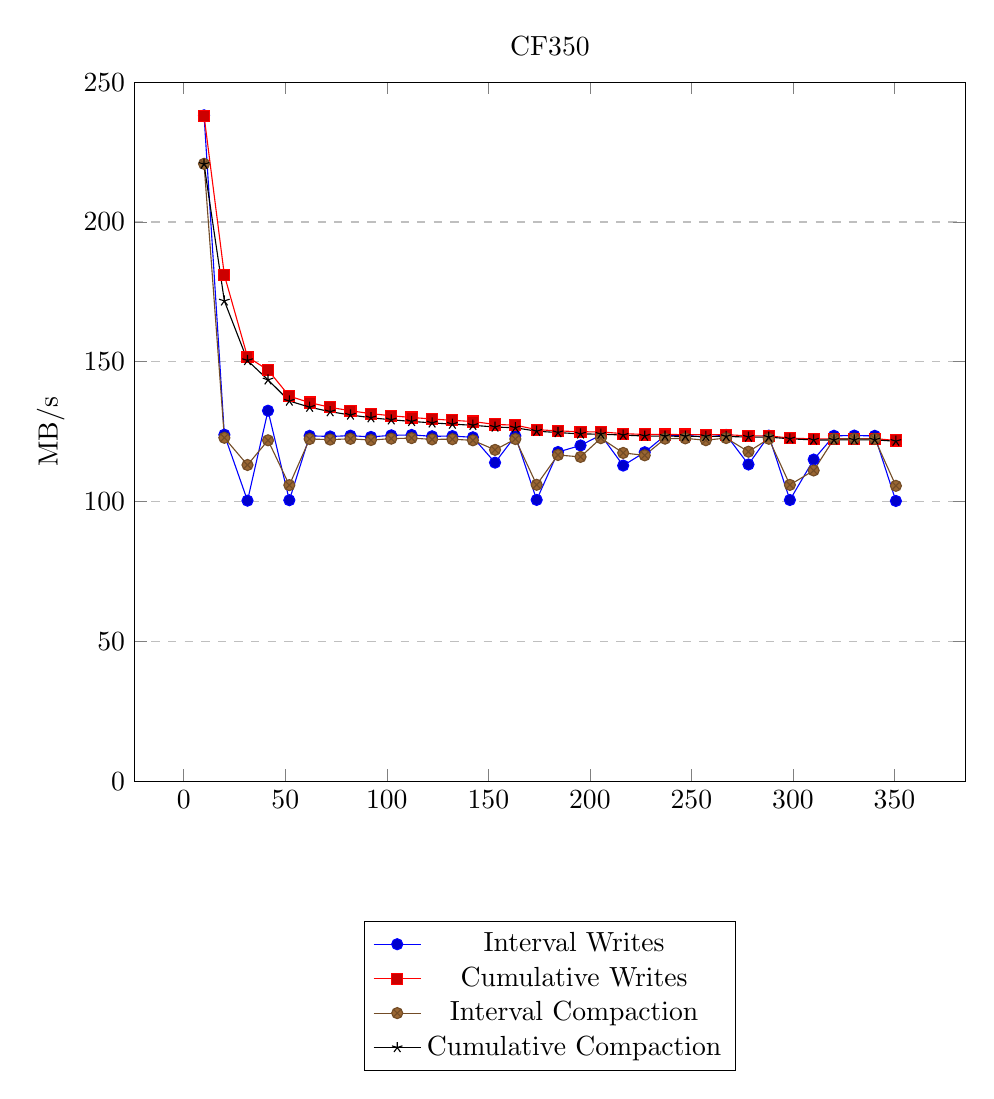
\begin{tikzpicture}
\begin{axis}[
    title=CF350,
    xlabel={},
    ylabel={MB/s},
    ymin=0,
    ymax=250,
    ytick={0,50,...,300},
    width=\textwidth,
    legend style={
        at={(0.5,-0.2)},
        anchor=north,legend columns=1
    },
    ymajorgrids=true,
    grid style=dashed,
]
\addplot
	coordinates { (10.0,238.15)(20.0,123.92)(31.4,100.32)(41.5,132.50)(52.0,100.48)(62.0,123.51)(72.1,123.28)(82.1,123.57)(92.2,123.12)(102.2,123.69)(112.2,123.82)(122.3,123.35)(132.3,123.41)(142.4,122.99)(153.3,113.92)(163.3,123.48)(173.8,100.59)(184.3,117.72)(195.4,120.06)(205.4,123.81)(216.4,112.87)(227.0,117.63)(237.0,123.61)(247.0,123.70)(257.1,123.04)(267.1,123.84)(278.1,113.26)(288.1,123.57)(298.5,100.55)(310.2,115.02)(320.2,123.53)(330.2,123.59)(340.3,123.51)(350.7,100.21) };
\addplot
	coordinates { (10.0,238.00)(20.0,181.00)(31.4,151.72)(41.5,147.05)(52.0,137.69)(62.0,135.40)(72.1,133.70)(82.1,132.47)(92.2,131.44)(102.2,130.68)(112.2,130.07)(122.3,129.52)(132.3,129.05)(142.4,128.62)(153.3,127.58)(163.3,127.33)(173.8,125.72)(184.3,125.27)(195.4,124.97)(205.4,124.91)(216.4,124.30)(227.0,123.99)(237.0,123.97)(247.0,123.96)(257.1,123.93)(267.1,123.92)(278.1,123.50)(288.1,123.51)(298.5,122.70)(310.2,122.42)(320.2,122.45)(330.2,122.49)(340.3,122.52)(350.7,121.85) };
\addplot
	coordinates { (10.0,220.80)(20.0,122.80)(31.4,113.08)(41.5,121.91)(52.0,105.87)(62.0,122.37)(72.1,122.16)(82.1,122.43)(92.2,121.99)(102.2,122.50)(112.2,122.69)(122.3,122.24)(132.3,122.30)(142.4,121.89)(153.3,118.48)(163.3,122.36)(173.8,105.99)(184.3,116.65)(195.4,115.97)(205.4,122.67)(216.4,117.39)(227.0,116.53)(237.0,122.49)(247.0,122.59)(257.1,121.94)(267.1,122.71)(278.1,117.83)(288.1,122.45)(298.5,105.96)(310.2,111.11)(320.2,122.41)(330.2,122.48)(340.3,122.39)(350.7,105.62) };
\addplot
	coordinates { (10.0,220.66)(20.0,171.76)(31.4,150.46)(41.5,143.53)(52.0,135.96)(62.0,133.76)(72.1,132.14)(82.1,130.96)(92.2,129.98)(102.2,129.24)(112.2,128.66)(122.3,128.13)(132.3,127.69)(142.4,127.28)(153.3,126.65)(163.3,126.39)(173.8,125.16)(184.3,124.68)(195.4,124.18)(205.4,124.11)(216.4,123.77)(227.0,123.43)(237.0,123.39)(247.0,123.36)(257.1,123.30)(267.1,123.28)(278.1,123.07)(288.1,123.04)(298.5,122.45)(310.2,122.02)(320.2,122.04)(330.2,122.05)(340.3,122.06)(350.7,121.57) };

\legend{Interval Writes, Cumulative Writes, Interval Compaction, Cumulative Compaction}
\end{axis}
    \end{tikzpicture}


\end{document}